%%%%%%%%%%%%%%%%%%%%%%%%%%%%
% Master's Thesis          %	    										
% Fabian Burth, 2022-08-01 %
%%%%%%%%%%%%%%%%%%%%%%%%%%%%

% Befehl für Anhang
\appendix

\chapter{Additional Information} \label{apx:AdditionalFigures}
\section{Black Duck Binary Analysis Result}
\begin{figure}[H]
	\centering
	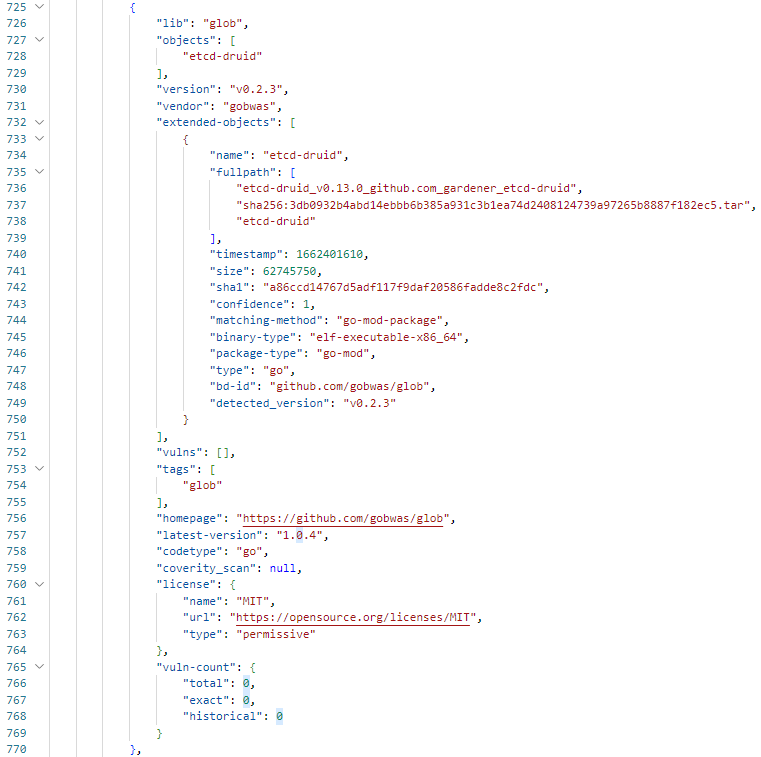
\includegraphics[width=0.9\textwidth]{bdbaResult}
	\caption[Snippet of BDBA Analysis Result]{Snippet of BDBA Analysis Result \source{\cite{BDBAIntegration}}}
	\label{fig:bdbaResult}
\end{figure}

\section{Relational Model of the Example Data Model Instance} \label{apx:Relational Model of the Example Data Model Instance}
This list shows a exemplary relational model corresponding to figure \ref{fig:RefDataModel} in section \ref{sec:Application of the Data Model}. The properties are deducted from the OCM, but as stressed several times, they are just one possible example. As this relational model is mainly supposed to support the general understanding of the problem domain, it treats each attribute as atomic. Thus, complex attributes such as repository context are not further normalized for the scope of this relational model.\par
\textit{Primary key attributes} are bold and underlined and \textit{foreign key attributes} are italic and underlined. Naturally, in this data model which rarely uses surrogate keys, but still has to represent several hierarchical relationships, attributes are frequently part of both, the primary and the foreign key.

\begin{itemize}
	\item \textbf{Component}(\textbf{\underline{name}})
	\item \textbf{ComponentVersion}(\textbf{\underline{\textit{name}}}, \textbf{\underline{version}}, labels, repository-context, provider)
	\item \textbf{ComponentReference}(\textbf{\underline{source-component-name}}, \textbf{\underline{source-component-version}}, \textbf{\underline{destination-component-name}}, \textbf{\underline{destination-component-version}}, \textbf{\underline{name}}, \textbf{\underline{extra-identity}}, labels)
	\item \textbf{Resource}(\textbf{\underline{name}}, \textbf{\underline{extra-identity}}, \textbf{\underline{\textit{component-name}}}, \textbf{\underline{\textit{component-version}}})
	\item \textbf{ResourceVersion}(\textbf{\underline{\textit{name}}}, \textbf{\underline{version}}, \textbf{\underline{\textit{extra-identity}}}, \textbf{\underline{\textit{component-name}}}, \textbf{\underline{\textit{component-version}}}, digest, labels, resource-type)
	\item \textbf{Source}(\textbf{\underline{name}}, \textbf{\underline{extra-identity}}, \textbf{\underline{\textit{component-name}}}, \textbf{\underline{\textit{component-version}}})
	\item \textbf{SourceVersion}(\textbf{\underline{\textit{name}}}, \textbf{\underline{version}}, \textbf{\underline{\textit{extra-identity}}}, \textbf{\underline{\textit{component-name}}}, \textbf{\underline{\textit{component-version}}}, labels)
	\item \textbf{IsBuiltFrom}(\textbf{\underline{component-name}}, \textbf{\underline{component-version}}, \textbf{\underline{resource-name}}, \textbf{\underline{resource-version}}, \textbf{\underline{resource-extra-identity}}, \textbf{\underline{source-name}}, \textbf{\underline{source-version}}, \textbf{\underline{source-extra-identity}})
	\item \textbf{Package}(\textbf{\underline{id}}, name)
	\item \textbf{PackageVersion}(\textbf{\underline{id}}, \underline{\textit{package-id}}, name, version, ecosystem, platform)
	\item \textbf{BDBAPackageVersion}(\textbf{\underline{name}}, \textbf{\underline{version}}, \underline{\textit{package-version-id}}, ecosystem, platform, matching-method)
	\item \textbf{SourceVersionIsComprisedOf}(\textbf{\underline{component-name}}, \textbf{\underline{component-version}}, \textbf{\underline{source-name}}, \textbf{\underline{source-version}}, \textbf{\underline{extra-identity}}, \textbf{\underline{package-version-id}})
	\item \textbf{ResourceVersionIsComprisedOf}(\textbf{\underline{component-name}}, \textbf{\underline{component-version}}, \textbf{\underline{resource-name}}, \textbf{\underline{resource-version}}, \textbf{\underline{extra-identity}}, \textbf{\underline{package-version-id}})
	\item \textbf{DependsOn}(\textbf{\underline{package-version-id}}, \textbf{\underline{package-version-id}})
	\item \textbf{Vulnerability}(\textbf{\underline{cve}}, summary, cvss, cwe)
	\item \textbf{Contains}(\textbf{\underline{package-version-id}}, \textbf{\underline{cve}})
\end{itemize}

The IsBuiltFrom-relationship contains a particularly interesting detail about this mapping. As explained in the respective sections, due to the \emph{Component Version-Local Identities} of \emph{Artifacts} in the OCM, \emph{Resource Versions} may only be built from \emph{Source Versions} within the same \emph{Component Version}. Thus, even though the component name and component version are part of the identities of both \emph{Source Version} and \emph{Resource Version}, it is only contained once in the IsBuiltFrom relation manifesting this (n:m)-relationship.\par
Another detail, of which the purpose may not be immediately obvious, are the surrogate keys, id, of \emph{Package Version} and \emph{Package}. The scanning tools and other data sources may use different identifiers for the same technical package or even identify different technical packages with the same identifier. Thus, the decision, that for example a \emph{BDBA Package Version} and a \emph{Mend Package Version} actually represent the same technical package has to be done by humans. Until then, the \emph{BDBA Package Version} and the \emph{Mend Package Version} have to be stored without merging and therefore relating to two different \emph{Package Versions} and \emph{Packages}. With natural keys, this could therefore lead to duplicate \emph{Package Versions} and \emph{Packages}.

\section{Relation of Number of Keys and Number of Leaves in a B-tree} \label{apx:Relation of Number of Keys and Number of Leaves in a B-tree}
Given $N+1$ is the number of leaf nodes of a B-tree. $n_{l} \epsilon  \mathbb{N}$ is the number of nodes on a particular level $l \epsilon \mathbb{N}$. Thereby, $l = 1$ is the lowest level, thus the leaf node level, and consequently $n_{1}$ is the number of leaf nodes, thus $n_{1} = N+1$. As a B-tree is a tree, it always has a root node. So $l = root$ is the highest level with $n_{l} = 1$.\par
As per constraint, the number of keys in a node is $k-1$. Since all the nodes on $l = 1$ are children of some node on $l = 2$ and every node on $l = 2$ has one key less than it has children, the total number of keys on $l_{2}$ is equal to $K_{2} = n_{1} - n_{2}$. This correlation is generally true, the number of keys on a level is equal to the number of nodes on the level below minus the number of nodes on the respective level (with the only exception of $l = 1$).
$$ K_{l} = n_{l-1} - n_{l} $$
The resulting sequence $(K_l)_{l=2}^{root}$ can be used to form a series calculating the cumulative number of keys up to a particular level.
$$\Sigma K_l = \Sigma_{i=2}^{l} n_{i-1} - n_{i} $$
And as every tree has a root node, $n$ always reaches $1$ at some point. This can be written as follows.
$$\Sigma K_{root} = (n_0 - n_1) + (n_1 - n_2) + (n_2 - n_3) + ... + (n_{l-1} - 1) $$
Obviously, all elements but the first, $n_0$, and the last, $1$, appear twice, once with a positive and once with a negative sign and thus reduce each other.
$$\Sigma K_{root} = n_0 - 1$$
And since $n_0 = N + 1$, the number of keys in a B-tree is

$$\Sigma K_{root} = N + 1 - 1 = N$$
